% Generated by documents/paper/figures/make_rq_appendix.py from the rq06_language_transfer README; do not edit.
\clearpage
\section{Language transfer}
\label{app:rq06_language_transfer}

\paragraph{Question.} If a language's BPB was measured on one or two small rungs only, can the exponent pooled over the other languages predict its BPB at the reference size, and does that hold for languages the model never trained on? Does a design decision a proxy reads on its trained languages carry over to the languages it did not train, and which languages must a developer evaluate to recover the multilingual decision?

\paragraph{Setup.} The language-list decision (scheme A vs B at $L \in \{8, 15, 30\}$, single-axis pairs, every seed) read on the bits per byte of 100 evaluation languages, grouped by whether both lists, one list or neither train the language and, if neither, whether they train its script. DA-size of the 90M--1B proxies and DA-ckpt of the 1.7B run's checkpoints, against the 1.7B final.

\paragraph{Key finding.} The list decision does not transfer to untrained languages at a proxy's scale: languages whose script a list trains are read at 0.63 (90M) and 0.72--0.73 (175M--600M), 0.81 only at 1B, and unseen scripts at 0.42--0.73, never 0.75. The languages the lists train are read at 0.77--1.00 (both lists) and 1.00 (one list). (Figure~\ref{fig:app_rq06_language_transfer}.)

\begin{figure}[h]
\centering
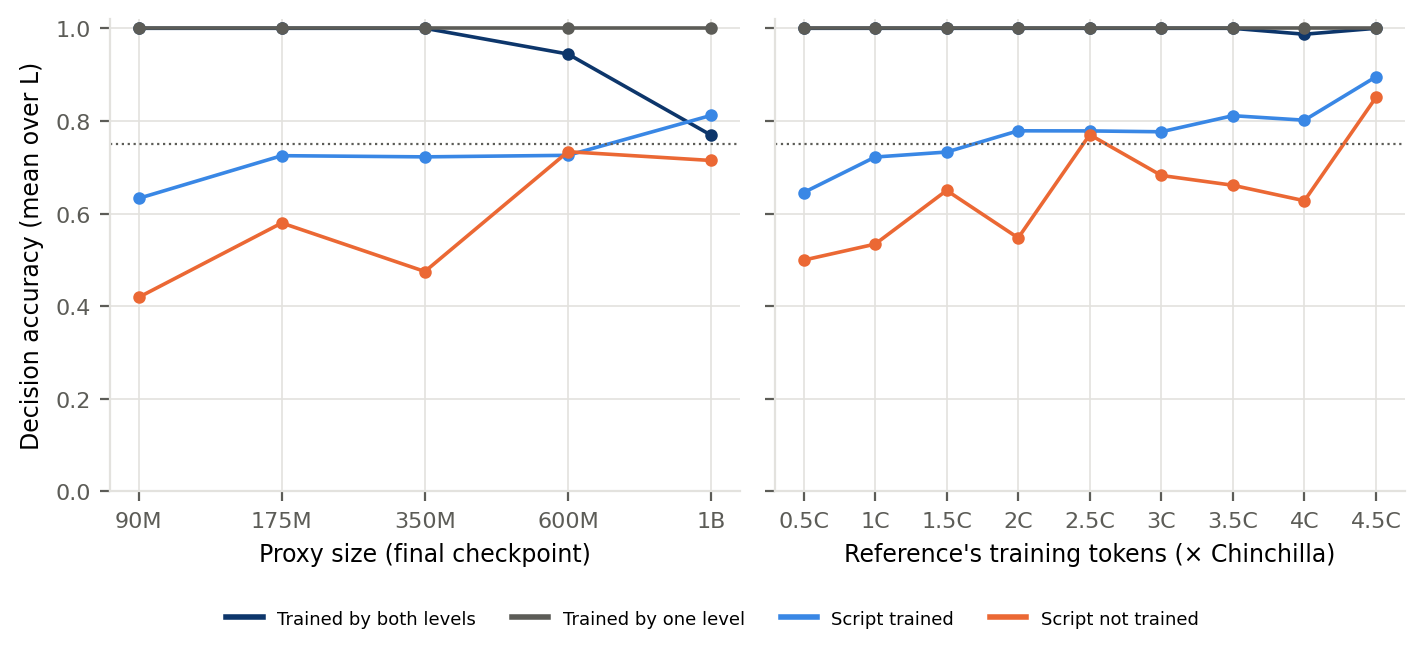
\includegraphics[width=\textwidth]{figures/app_language_transfer.png}
% source: src/signal-and-noise/analysis/rq06_language_transfer/pretraining/predictivity_seeds/transfer_da_all_lines_mono_axis_paper.png
\caption{The list decision by language group, by proxy size and by the reference's checkpoints.}
\label{fig:app_rq06_language_transfer}
\end{figure}
